\documentclass[a4paper,12pt]{article}

%% Language and font encodings
\usepackage[english]{babel}
\usepackage[utf8x]{inputenc}
\usepackage[T1]{fontenc}

%% Sets page size and margins
\usepackage[a4paper,top=3cm,bottom=2cm,left=3cm,right=3cm,marginparwidth=1.75cm]{geometry}

%% Useful packages
\usepackage{amsmath}
\usepackage{graphicx}
\usepackage{hyperref}

\title{IGR203 project report}
\author{Alexis Bauvin -- Clément Decoodt -- Ronan Desplanques -- Ming Yang}

\begin{document}
\maketitle

\tableofcontents

\section*{Introduction}

The project we chose is the interactive restaurant menu. Indeed, this project gives us a lot of freedom of movement
in the creation of the design.

This project aims to design an interactive menu for a restaurants to be given to customers. We designed this project
with two objectives in mind : a tablet app, given to the seated client by the waiter and a smartphone app for an
outside client, wanting to order remotely.

\newpage

\section{The design}

\subsection{The overseen leads}

\subsubsection{Tablet-oriented design}

The first lead is a design thought for a tablet. It uses the whole screen estate of this platform to provide an
pleasant and original interface, while being practical. Metaphors are being used all over the design that recall
traditional restaurant menus. Furthermore, the middle of the interface gives the current state of the order by taking
the form of a restaurant table where chosen items appear on the table.

\subsubsection{Smartphone-oriented design}

This design idea relates to a smartphone implementation. On a rather small screen, it emphasises on simplicity and
clarity by using a list interface. Buttons are large and do occupy the whole screen, with greatly reduced decorative
clutter.

\subsubsection{Traditional design}

The foundation of this design is the idea to emulate as much as possible a classical menu. The main part of the
interface takes the shape of the traditional menu. It is only by touching an element that one can access extra
information and order. To increase the "paper" aspect of the interface, we recycle the characteristics of
e-readers such as curling page animations and background color.

\subsection{The chosen one}

In the end, the first design has been chosen for the main interface. It is the one to provide the most added value
against a traditional approach. Moreover, implementation-specific constraints do not look impossible to overtake.
Needs in interaction and personnalisation of the interface are answered by the design. This design is intuitive and
does not have any learning curve before being useful: tha "recognition over recall" principle is kept.

However, this design diverges from portability requirements: to be experienced to its maximum, the interface needs to
be laid out on a large screen. And by large, it is both physical size and definition. Thus, the interface needs at
least a tablet to be efficient. It is not aimed to be used by clients on their own phones.

Regarding this last point, an alternative version of the interface, more streamlined, following the second design,
will be implemented.

\subsection{Evolutions of the needs along the design}

Combining all different use needs in an unique designed proved not to be possible. The difficulty was to offer
attractive enough features to justify a swith to a fully digital menu system for on-place clients. Furthermore, it
could event be adapted to be used on the personal devices of the clients.

Our solution is to offer two interactive clients. Most of the development should be dedicated to the main tablet
interface. However, this does not results in a redundancy in the whole system because all the logic is shared between
the tablets.

\subsection{Design mechanics}

Here, we will dicuss all the details of the main chosen interface and its workings : interactions, concepts, ...

\subsubsection{Introduction screen}

The introduction screen is shown to the user at the very beginning of his interaction with the system. He is lead to
choose between "On place" or "Takeaway" to place his order. Although the default language is French, a button
looking like a flag is placed in a corner. It allows to change the language of the app.

\begin{center}
	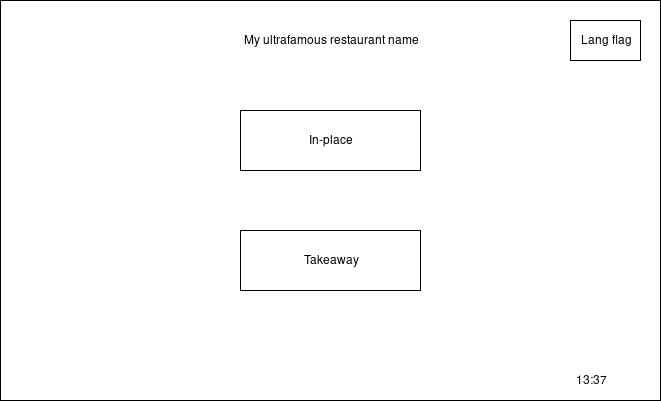
\includegraphics[width=\textwidth]{intro_screen.jpg}
\end{center}

Another layout was also considered :

\begin{center}
	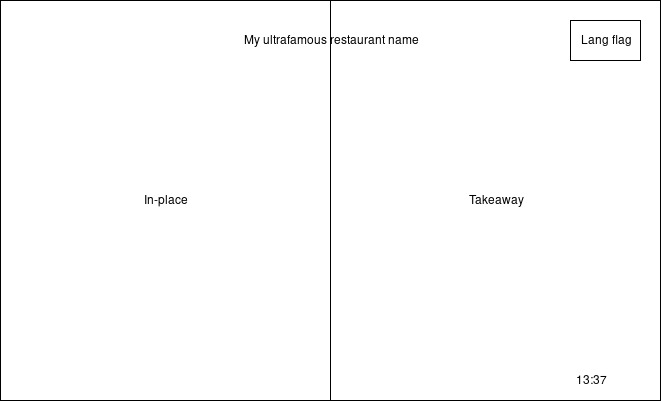
\includegraphics[width=\textwidth]{alt_intro_screen.jpg}
\end{center}

This is the final layout, as it is warmer to the user while being more efficient by reducing the precision needed to
transition to the next screen.

\subsubsection{The "on place" screen}

This part of the user interface relies on two card "decks": one at the bottom of the screen and the other on the
right. The right-hand one allows to choose the desired menu category, mapped to an article type. These may include
starters, main courses, drinks, ... whose contents will be "sent" to the bottom deck. The bottom deck is used to
choose an article in a category, like a \emph{coq au vin}\footnote{En français dans le texte}. The flag button stays
on-screen here, as well as on every other screen.

\begin{center}
	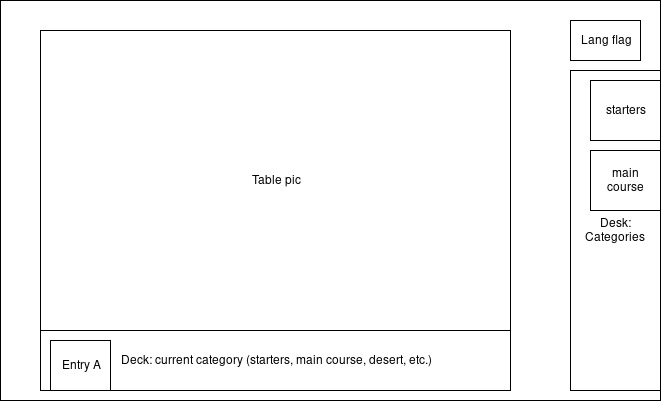
\includegraphics[width=\textwidth]{in_place_screen1.jpg}
\end{center}

A click -- or tap -- on an article, a modal screen pops in and displays details about the article, and allows to
give more insighst on an element (gluten free, vegan, ...) before adding it to the order.

\begin{center}
	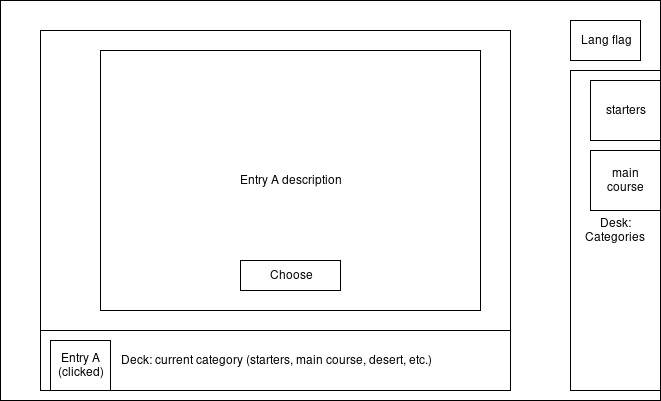
\includegraphics[width=\textwidth]{in_place_screen2.jpg}
\end{center}

Selecting an item is done through a "card deck" concept: each card represents an element, that one adds by dragging
it. Adding a dish -- or any other article -- to the order is a matter of dragging a card to the center of the screen,
dropping it on the table picture.

\begin{center}
	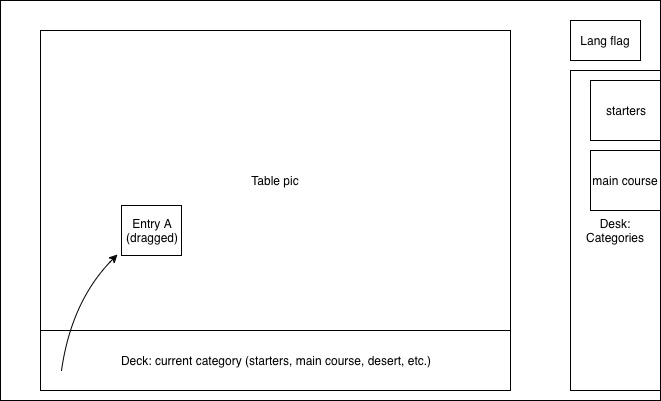
\includegraphics[width=\textwidth]{in_place_drag.jpg}
\end{center}

This mechanics remains the same one to change the menu category. One drags a card from the right-hand deck (let's
say "starters"), then drags it to the bottom of the screen, then drops it on the bottom deck. This will spread the
stack of cards representing the items of this category.

The middle of the screen is filled by table picture, allowing the customer to view his order "visually": as he adds
items to his order, the table fills up with elements he orders.

The drag-and-drop system allows an intuitive and streamlined choice mechanic. Let's take the example of a steak:
it is crucial that the client is able to choose the cooking -- although "well done" should be banned. When a card
has different options -- here "Rare", "Medium rare", "Well done" --, transparent overlays appear over the table.
There are as many as there is options for this item, each mapping to an option. In our example, three boxes would be
available : "Rare", "Medium rare", "Well done". The registered option will be the one the client drops the card on.

\begin{center}
	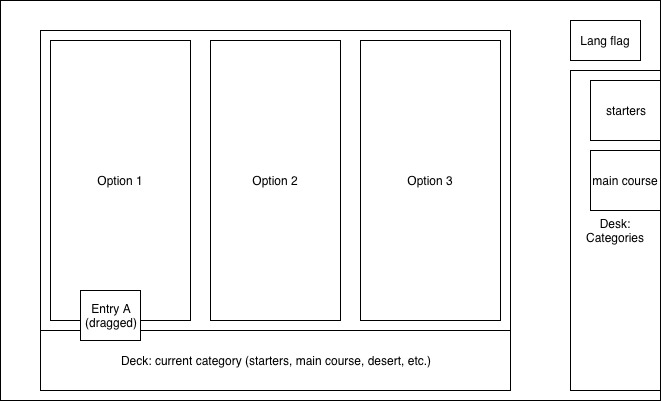
\includegraphics[width=\textwidth]{in_place_drag_options.jpg}
\end{center}

\subsubsection{The "takeaway" screen}

Because users ordering with takeaway may be more speedy than those in the restaurant, the interface is simpler and
more practical. Items are laid out in a simple hierarchical list with sub-categories. However, the modal system from
the "on place" takes a big role here.

\begin{center}
	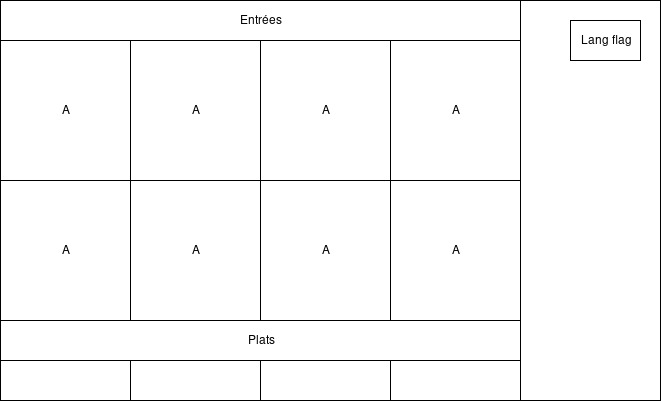
\includegraphics[width=\textwidth]{takeaway_screen.jpg}
\end{center}

\subsubsection{Confirmation screen}

After validating the order, a new screen displays a summary of the order and prompts the user to confirm the order.

\begin{center}
	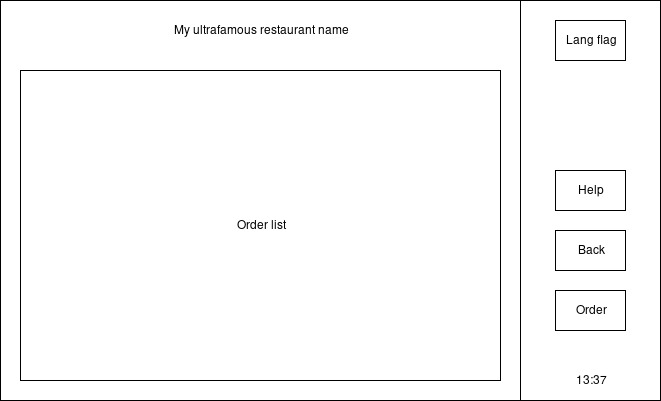
\includegraphics[width=\textwidth]{confirmation_screen.jpg}
\end{center}

\subsubsection{Final screen}

After confirming the order, a thank you screen takes place. There, an estimate of the waiting time is displayed
before the dishes to be served. An additional field is available if the client has a special request for the
restaurant.

\begin{center}
	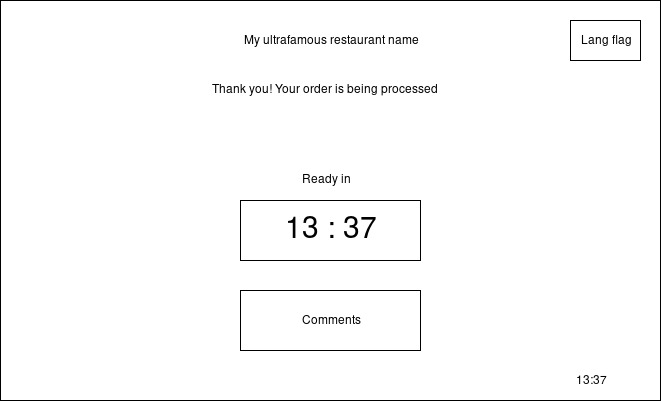
\includegraphics[width=\textwidth]{final_screen.jpg}
\end{center}

\section{Prototype}

\subsection{Practical informations}

All the source code for the prototype is hosted on GitHub at the following address: \\
\url{https://github.com/friendshipismagic/pinkie-card.git}.

This prototype was accomplished thanks to the Qt framework for several reasons. Mainly, we were all familiar with this
toolkit to a certain degree. Furthermore, compared to iOS or Android, it is the only one excluding nobody from the
group for not having the right hardware -- either an iPad and a Mac or an Android tablet.

\subsection{Advancement}

It is relatively easy to follow the advancement of the prototype: the GitHub repository should speak by himself.
But, for the sake of completeness, here it is: the prototype is well advanced, though it still is a dumb prototype,
and it still lacks a few features.

Please note that the most up-to-date branch may not be \texttt{master} but \texttt{develop}.

\section{Analysis and research}

In order to indentify the needs of customers, we chose to interview customers directly at restaurants. This was the
preferred method since we can pinpoint more precisely requests from different ranks, classes, professions,
personalities, ... Furthermore, it is more amiable and friendly. We interviewed several persons from age 18 to 40.
Here are two personas and scenarios we could extract from these interviews :

\subsection{Antoine Dubois}

\begin{itemize}

\item Age - 27
\item Activity - Web designer
\item Interests - technology, social networking, modern popular culture.
\item Skills - good communication, used to traditional user interfaces, open-mindedness.
\item Lives in the city.
\item Restaurant habits - regularly eats in both traditional and modern-style restaurants. Is very receptive to
	presentation, appearance and atmosphere. Not reluctant to use technology at all, even in uncommon situations.
	Tend to appreciate traditional restaurant features more and more as he grows older.
\item Associated scenario - He has heard about the ordering system through promotion. He comes with some friends
	who have somewhat similar interests and they intend to discuss the system and lay a critical eye on it. They are
	on the advanced side of the user spectrum and use the devices easily, but feel like it could be less detailed
	(e.g. they find the help tips unhelpful because stating the obvious). After orders are taken conversation
	completely changes subject. He expected more innovative features as he is interested in what can be done with
	user interfaces and is not satisfied with simply not noticing it.

\end{itemize}

\subsection{Julien Deschamps}

\begin{itemize}

\item Age: 20
\item Activity: Student
\item Interests: music, drawing
\item Restaurant habits: Used to modern burger restaurants and Kebab/pizza style. Used to Domino's pizza web interface
\item Associated scenario: Julien is going to his favorite kebab restaurant, the `France Gourmet`. While he's still
	in his bedroom, he uses the Android App to pre order his kebab. In less than a minute, his command is being
	processed. He's finishing his homeworks, while his phone is notifying him, saying that the kebab will be available
	in 5 minutes. He then goes to the restaurant, and meets Grégoire. Grégoire is also going to order a kebab, so
	they'll eat it together in the park in front of the restaurant. They both go to the restaurant. Julien's kebab
	is ready to go, Grégoire will have to wait another minute (he arrived a little earlier). Their payment is already
	done via the app, they can just go outside and eat!

\end{itemize}

\subsection{Lessons leared}

Some of them are familiar with ordering systems, while a number of them are not used to it and tend to appreciate
more tranditional restaurant features. Some of them enjoy their meal with their friends or families inside the
restaurant, while some are in hurry and choose to take away. Considering of these situations, we choose to design
2 different ordering systems. One system is for those who eat inside and the other is for those who choose to take
away. For those who eat at restaurant, details of each dish should be more precise and it is better with a vivid
picture of each dish shown on the screen. For those who choose to take away, the interface should be more simple
and functional. Besides we want our design to be fun. We hope that our customers want to discover and explore our
interface. We want our customers’ ordering experience to be unique and joyful. So we decide to merge cards into the
interface so that ordering is like a card game. Moreover, we want our design to be accessible to people from all
ages. That is to say, whether the old or children, they can make ordering by themselves. So it requires our design
to be as simple as possible. And also we should simplify the ordering steps and make every step clear to customers.

\end{document}

